\section{Accelerometer}
Idéer til accelerometer:
\begin{description}[style=nextline]
\item Gangart
\item Rystelser
\item Aktivitetsniveau
\item Nattesøvn
\end{description}

Sensor
\begin{description}[style=nextline]
\item[Kan vi få fat i data?] Ja, de er tilgængelig fra MotionSensor.
\item[Er der begrænsninger?] Umiddelbart ingen begrænsninger.
\item[Hvilke data giver sensoren?] Acceleration i x,y,z akserne.
\end{description}

Analyse
\begin{description}
\item[Har vi data nok?] Til gangart tror vi ikke der er data nok, men til rystelser og aktivitetsniveau er der nok til at analysere på. Til nattesøvn er der allerede flere applikationer som implementere dette, så det er også muligt.
\item[Hvilke data skal benyttes?] For gangart skal man muligvis også benytte gyro sensor i sammensættelse med acceleration endvidere kan det være at man skal vide hvilken retning tyngdekræften trækker. Til rysteler og aktivitetsniveau er det nok med at bare bruge accelerometer, da vi baseret på den kan se om de bevæger telefonen(Dog med at i nogle situationer kan brugeren snyde hvis de bare leger med telefonen meget), det er nok svære at se hvor meget de nu bevæger sig(f.eks om de løber eller går). 
\item[Formål med analysen] Baseret på det vi har hørt fra Morten, er motion og aktivitet vigtigt for personer med psykiske sygdomme og hvis de ikke rører på sig særlig meget kan det være en indikator for hvilken slags sinds situation de befinder sig i.
\item[Ide til visualisering (?)] Normal 2 dimensionel graf som viser aktivitets niveau over flere dage, uger, måneder. Muligivis en kalender der hvis hvor aktiv man har været på en bestemt dato, så en dato man har været meget aktiv er grøn, og en dato hvor man har været meget lidt aktiv er datoen rød.
\item[(kort oprids af fremgangsmåde)] Hvis man laver grafen skal man tage man målinger om dagen og så lav et gennemsnit på det ved enden af dagen og tilføje det til grafen.
\item[(gem illustrationer og kilder)] 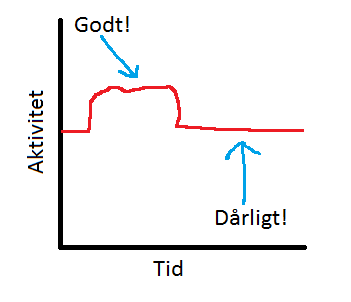
\includegraphics{aktivitet_billed}
\end{description}